% XCircuit output "sna_limesdr.tex" for LaTeX input from sna_limesdr.ps
\def\putbox#1#2#3#4{\makebox[0in][l]{\makebox[#1][l]{}\raisebox{\baselineskip}[0in][0in]{\raisebox{#2}[0in][0in]{\scalebox{#3}{#4}}}}}
\def\rightbox#1{\makebox[0in][r]{#1}}
\def\centbox#1{\makebox[0in]{#1}}
\def\topbox#1{\raisebox{-0.60\baselineskip}[0in][0in]{#1}}
\def\midbox#1{\raisebox{-0.20\baselineskip}[0in][0in]{#1}}
   \scalebox{1}{
   \normalsize
   \parbox{4.39583in}{
   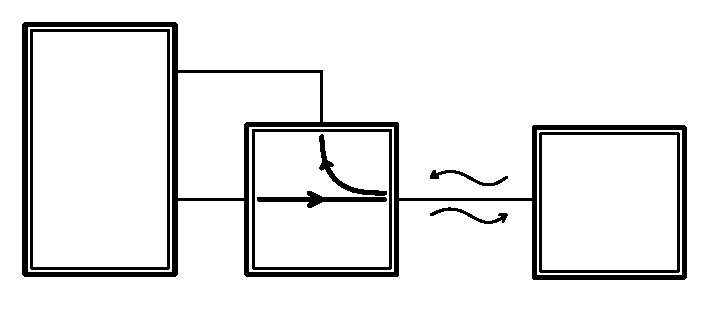
\includegraphics[scale=1]{sna_limesdr}\\
   % translate x=76 y=390 scale 0.38
   \putbox{2.99in}{0.42in}{1.20}{\centbox{Incident}}%
   \putbox{2.99in}{0.23in}{1.20}{\centbox{power $P_i$}}%
   \putbox{3.01in}{1.21in}{1.20}{\centbox{Reflected}}%
   \putbox{3.01in}{1.02in}{1.20}{\centbox{power $P_r$}}%
   \putbox{2.06in}{1.07in}{1.20}{$X~\mr{dB}$}%
   \putbox{2.06in}{1.52in}{1.20}{\midbox{$P_s=P_r-X$}}%
   \putbox{3.95in}{0.75in}{2.40}{\centbox{\midbox{DUT}}}%
   \putbox{2.06in}{0.09in}{1.20}{\centbox{Directional coupler}}%
   \putbox{0.54in}{1.09in}{1.80}{\rotatebox{-270}{\centbox{\midbox{LMS7002M}}}}%
   \putbox{0.97in}{0.75in}{1.20}{\rightbox{\midbox{Tx}}}%
   \putbox{0.97in}{1.61in}{1.20}{\rightbox{\midbox{Rx}}}%
   } % close 'parbox'
   } % close 'scalebox'
   \vspace{-\baselineskip} % this is not necessary, but looks better
